\documentclass[color=usenames]{beamer}
\mode<presentation>

\usetheme{Frankfurt}
%\usepackage{times}
\usepackage[utf8]{inputenc}  %% 1
\usepackage[T2A]{fontenc}      %% 2
\usepackage[russian]{babel}    %% 3
\usepackage{multirow}

\renewcommand{\vec}[1]{\boldsymbol{#1}}
\newcommand{\HL}{\mathcal{L}}
\newcommand{\HH}{\mathcal{H}}

\begin{document}

\title{MathGL -- библиотека для научной графики}

\author{A.A. Балакин}
%\institute{Институт прикладной физики РАН, Н.Новгород, Россия}

\date{\flushleft
\textbf{MathGL это \ldots}\\
качественная научная графика на различных ОС (Windows, Linux, MacOS);\\
быстрая обработка и отображение больших массивов данных;\\
работа в графическом и консольном режимах;\\
легкое интегрирование в другие программы;\\
большой и обновляемый набор графиков и инструментов обработки данных.
}

\begin{frame}
\titlepage
\end{frame}

\section{MathGL Overview}

\begin{frame}{Обзор MathGL}
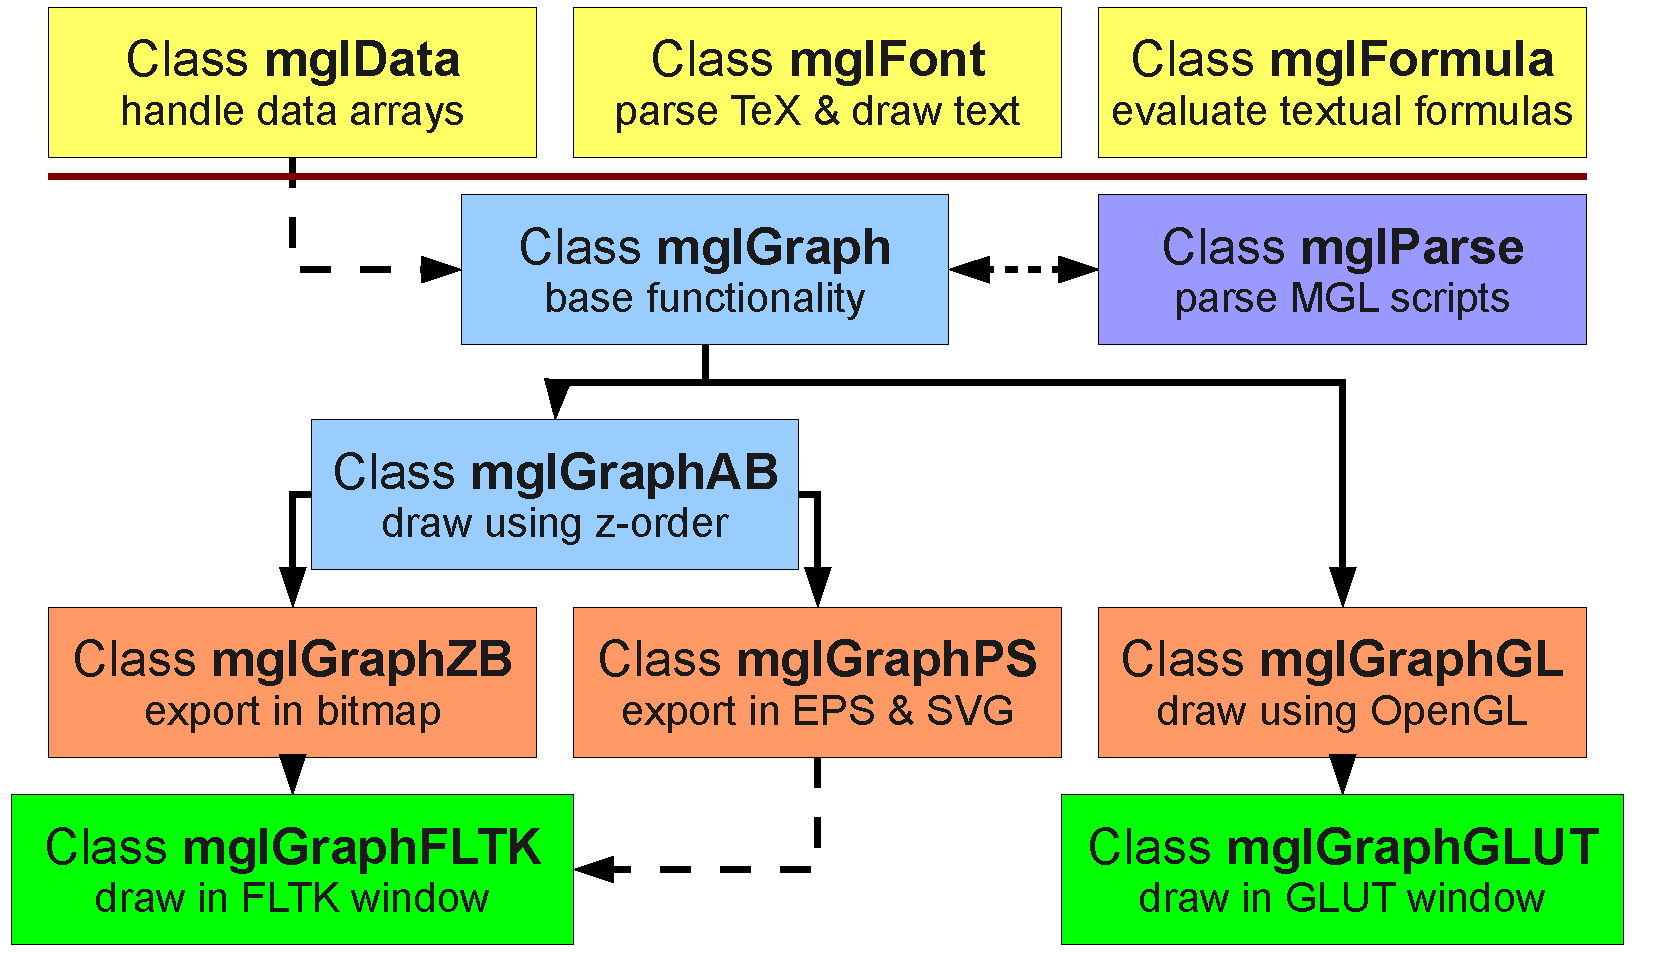
\includegraphics[width = \textwidth]{classes}
\end{frame}

\begin{frame}{Вывод текста}
\includegraphics[width = \textwidth]{png/sample4_lg.png}
\end{frame}

\begin{frame}{Оси координат}
\begin{columns}
\column{0.5\textwidth}
Криволинейные координаты.\\
\includegraphics[width = \textwidth]{png/sample3_lg.png}

Логарифмические оси\\
\includegraphics[width = \textwidth]{png/loglog_lg.png}

\column{0.5\textwidth}
Несколько осей\\
\includegraphics[width = \textwidth]{png/2_axis_lg.png}

Легенда графика\\
\includegraphics[width = \textwidth]{png/legend_lg.png}

\end{columns}
\end{frame}

\begin{frame}{Возможности экспорта}
\begin{itemize}
\item Экспорт в растровый рисунок PNG, JPEG, GIF
\item Экспорт в векторный рисунок EPS или SVG
\item Рисование во встроенном окне GLUT или FLTK
\item Рисование во внешней программе как bitmap
\end{itemize}
\begin{columns}
\column{0.5\textwidth}
\includegraphics[width = \textwidth]{png/surf_lg.png}

\column{0.5\textwidth}
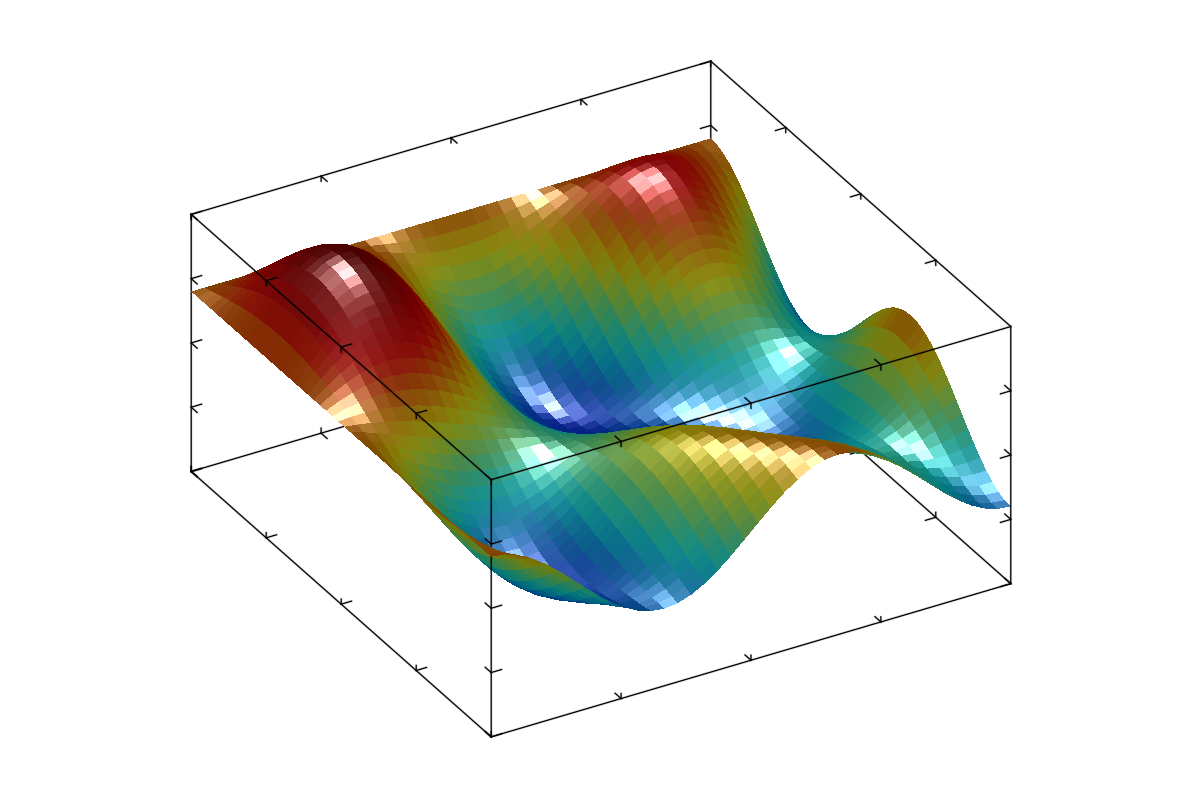
\includegraphics[width = \textwidth]{png/surf_eps.png}
\end{columns}
\end{frame}


\begin{frame}{Положение графика}
\begin{columns}
\column{0.5\textwidth}
\includegraphics[width = \textwidth]{png/sample1_lg.png}\\
\includegraphics[width = \textwidth]{png/ternary_lg.png}

\column{0.5\textwidth}
\includegraphics[width = \textwidth]{png/column_lg.png}\\
\includegraphics[width = \textwidth]{png/stick_lg.png}

\end{columns}
\end{frame}

\begin{frame}{Стерео изображение}
\includegraphics[width = \textwidth]{png/stereo_lg.png}
\end{frame}


\begin{frame}{Цвета}
\begin{columns}
\column{0.5\textwidth}
Цвета задаются символами (буквами). В цветовой схеме можно менять яркость (т.н. символ цвета с цифрой). MathGL по умолчанию использует следующие цвета.\\
\includegraphics[width = \textwidth]{png/colors_lg.png}

\column{0.5\textwidth}
Цветовая схема задается строкой с символами цвета. Символ '|' отключает сглаживание цвета.\\
\includegraphics[width = \textwidth]{png/color_schemes_lg.png}
\end{columns}
\end{frame}

\begin{frame}{Стили линий}
\begin{columns}
\column{0.5\textwidth}
Стили линий и маркеры также задаются символами.\\
\includegraphics[width = \textwidth]{png/sample5_lg.png}

\column{0.5\textwidth}
Стрелки можно нарисовать на концах кривой. Первый символ -- стрелка в конце, второй -- в начале кривой.\\
\includegraphics[width = \textwidth]{png/sampled_lg.png}
\end{columns}
\end{frame}

\begin{frame}{Скрипты MGL}
\begin{itemize}
\item Команды -- текстовые строки
\item Широкий спектр графиков и возможностей обработки данных
\item Простая структура языка
\item Экспорт в растровые (PNG, JPEG, GIF) или векторные (EPS, SVG) файлы
\item Нет компиляции
\item WYSWYG и утилиты командной строки
\end{itemize}

\begin{columns}\small
\column{0.5\textwidth}
\texttt{\flushleft
plot dat; xrange 0 1\\
box: axis\\
xlabel 'x': ylabel 'y'\\
\# Use cycle for lines\\
for \$0 -1 1 0.1\\
line 0 0 -1 \$0 'r'\\
next}

\column{0.5\textwidth}
\includegraphics[width = \textwidth]{png/parser_lg.png}
\end{columns}
\end{frame}

\begin{frame}{UDAV}
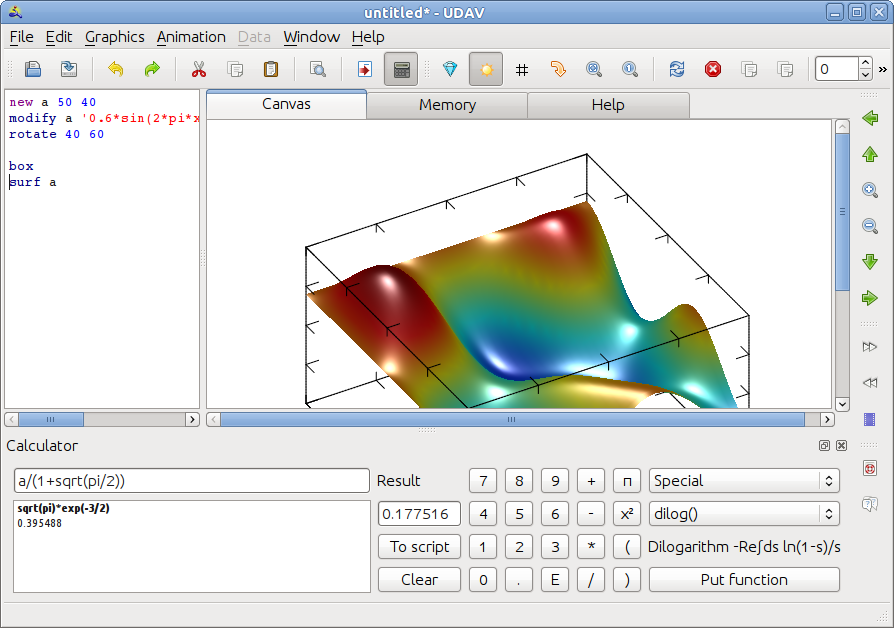
\includegraphics[width = \textwidth]{main.png}
\end{frame}

\begin{frame}{Графика в окне FLTK}
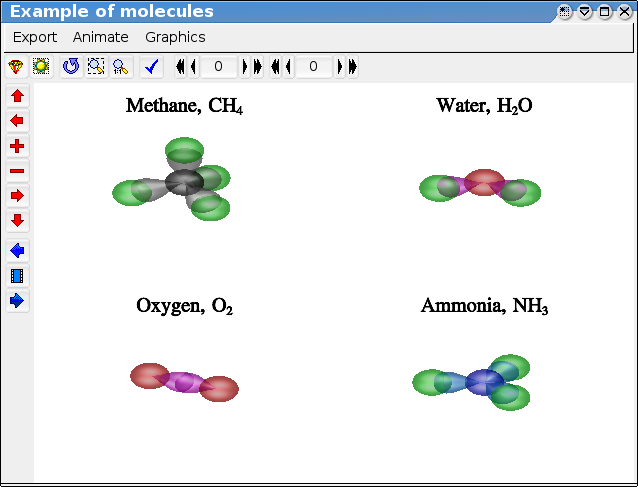
\includegraphics[width = 0.9 \textwidth]{fltk.png}
\end{frame}


\section{1D data}

\begin{frame}{Plot, Step, Tube}
\begin{columns}
\column{0.5\textwidth}
\includegraphics[width = \textwidth]{png/plot_lg.png}\\
\includegraphics[width = \textwidth]{png/step_lg.png}

\column{0.5\textwidth}
\includegraphics[width = \textwidth]{png/tube_lg.png}\\
\includegraphics[width = \textwidth]{png/tube_3d_lg.png}

\end{columns}
\end{frame}

\begin{frame}{Area, Stem, Region}
\begin{columns}
\column{0.5\textwidth}
\includegraphics[width = \textwidth]{png/area_lg.png}\\
\includegraphics[width = \textwidth]{png/area_2_lg.png}

\column{0.5\textwidth}
\includegraphics[width = \textwidth]{png/stem_lg.png}\\
\includegraphics[width = \textwidth]{png/region_lg.png}

\end{columns}
\end{frame}

\begin{frame}{Bars}
\begin{columns}
\column{0.5\textwidth}
\includegraphics[width = \textwidth]{png/bars_lg.png}\\
\includegraphics[width = \textwidth]{png/barh_lg.png}

\column{0.5\textwidth}
\includegraphics[width = \textwidth]{png/bars_2_lg.png}\\
\includegraphics[width = \textwidth]{png/bars_a_lg.png}

\end{columns}
\end{frame}

\begin{frame}{Error, Mark, BoxPlot}
\begin{columns}
\column{0.5\textwidth}
\includegraphics[width = \textwidth]{png/error_lg.png}\\
\includegraphics[width = \textwidth]{png/boxplot_lg.png}

\column{0.5\textwidth}
\includegraphics[width = \textwidth]{png/mark_lg.png}\\
\includegraphics[width = \textwidth]{png/textmark_lg.png}

\end{columns}
\end{frame}

\begin{frame}{Chart, Torus}
\begin{columns}
\column{0.5\textwidth}
\includegraphics[width = \textwidth]{png/chart_lg.png}\\
\includegraphics[width = \textwidth]{png/pie_chart_lg.png}

\column{0.5\textwidth}
\includegraphics[width = \textwidth]{png/ring_chart_lg.png}\\
\includegraphics[width = \textwidth]{png/torus_lg.png}

\end{columns}
\end{frame}


\section{2D data}

\begin{frame}{Surf}
\begin{columns}
\column{0.5\textwidth}
\includegraphics[width = \textwidth]{png/surf_lg.png}\\
\includegraphics[width = \textwidth]{png/surf_alpha_lg.png}

\column{0.5\textwidth}
\includegraphics[width = \textwidth]{png/surf_cont_fog_lg.png}\\
\includegraphics[width = \textwidth]{png/surf_cont_y_lg.png}

\end{columns}
\end{frame}

\begin{frame}{Dens, Cont, Mesh}
\begin{columns}
\column{0.5\textwidth}
\includegraphics[width = \textwidth]{png/dens_lg.png}\\
\includegraphics[width = \textwidth]{png/contt_lg.png}

\column{0.5\textwidth}
\includegraphics[width = \textwidth]{png/cont_lg.png}\\
\includegraphics[width = \textwidth]{png/mesh_lg.png}

\end{columns}
\end{frame}

\begin{frame}{Boxs, Tile, ContF, Belt}
\begin{columns}
\column{0.5\textwidth}
\includegraphics[width = \textwidth]{png/boxs_lg.png}\\
\includegraphics[width = \textwidth]{png/tile_lg.png}

\column{0.5\textwidth}
\includegraphics[width = \textwidth]{png/contf_lg.png}\\
\includegraphics[width = \textwidth]{png/belt_lg.png}

\end{columns}
\end{frame}

\begin{frame}{SurfC, SurfA, TileS, Axial}
\begin{columns}
\column{0.5\textwidth}
\includegraphics[width = \textwidth]{png/surfc_lg.png}\\
\includegraphics[width = \textwidth]{png/surfa_lg.png}

\column{0.5\textwidth}
\includegraphics[width = \textwidth]{png/tiles_lg.png}\\
\includegraphics[width = \textwidth]{png/axial_lg.png}

\end{columns}
\end{frame}


\section{3D data}

\begin{frame}{Surf3}
\begin{columns}
\column{0.5\textwidth}
\includegraphics[width = \textwidth]{png/surf3_lg.png}\\
\includegraphics[width = \textwidth]{png/dens_xyz_lg.png}

\column{0.5\textwidth}
\includegraphics[width = \textwidth]{png/cutminmax_lg.png}\\
\includegraphics[width = \textwidth]{png/cutminmax2_lg.png}

\end{columns}
\end{frame}

\begin{frame}{Cloud, Dens3, Cont3, ContF3}
\begin{columns}
\column{0.5\textwidth}
\includegraphics[width = \textwidth]{png/cloud_lg.png}\\
\includegraphics[width = \textwidth]{png/densa_lg.png}

\column{0.5\textwidth}
\includegraphics[width = \textwidth]{png/conta_lg.png}\\
\includegraphics[width = \textwidth]{png/contfa_lg.png}

\end{columns}
\end{frame}

\begin{frame}{Surf3C, Surf3A, Dots, Crust}
\begin{columns}
\column{0.5\textwidth}
\includegraphics[width = \textwidth]{png/surf3c_lg.png}\\
\includegraphics[width = \textwidth]{png/surf3a_lg.png}

\column{0.5\textwidth}
\includegraphics[width = \textwidth]{png/dots_lg.png}\\
\includegraphics[width = \textwidth]{png/crust_lg.png}

\end{columns}
\end{frame}


\section{Vector fields}

\begin{frame}{Vect, Traj}
\begin{columns}
\column{0.5\textwidth}
\includegraphics[width = \textwidth]{png/vect_lg.png}\\
\includegraphics[width = \textwidth]{png/vectc3_lg.png}

\column{0.5\textwidth}
\includegraphics[width = \textwidth]{png/vectc_lg.png}\\
\includegraphics[width = \textwidth]{png/traj_lg.png}

\end{columns}
\end{frame}

\begin{frame}{Flow, Pipe}
\begin{columns}
\column{0.5\textwidth}
\includegraphics[width = \textwidth]{png/flow_lg.png}\\
\includegraphics[width = \textwidth]{png/flow3_lg.png}

\column{0.5\textwidth}
\includegraphics[width = \textwidth]{png/pipe_lg.png}\\
\includegraphics[width = \textwidth]{png/pipe3_lg.png}

\end{columns}
\end{frame}


\section{Data handling}
\begin{frame}{Обработка данных (mglData)}
\Large
\begin{itemize}
\item Данные могут иметь до 3 размерностей: $a_{ijk}$
\item Безопасное выделение/освобождение памяти
\item Чтение/запись текстовых файлов, включая сжатые
\item Чтение/запись файлов HDF4 и HDF5 
\item Заполнение равномерно или по формуле
\item Сглаживание, дифференцирование, интегрирование, ...
\item Поиск максимумов, минимумов, моментов, ...
\item Выделение под-массивов, сумм, распределений, ...
\item и т.д.
\end{itemize}
\end{frame}

\begin{frame}{Fitting, Envelop, Sewing, ...}
\begin{columns}
\column{0.5\textwidth}
\includegraphics[width = \textwidth]{png/fit_lg.png}\\
\includegraphics[width = \textwidth]{png/envelop_lg.png}

\column{0.5\textwidth}
\includegraphics[width = \textwidth]{png/sew_lg.png}\\
\includegraphics[width = \textwidth]{png/sample6_lg.png}

\end{columns}
\end{frame}

\begin{frame}{PDE, Smoothing, STFA}
\begin{columns}
\column{0.5\textwidth}
\includegraphics[width = \textwidth]{png/pde_lg.png}\\
\includegraphics[width = \textwidth]{png/qo2d_lg.png}

\column{0.5\textwidth}
\includegraphics[width = \textwidth]{png/sample7_lg.png}\\
\includegraphics[width = \textwidth]{png/stfa_lg.png}

\end{columns}
\end{frame}

\section{Conclusion}
\begin{frame}{Заключение}
\LARGE
Посетите страницу MathGL\\[18pt]

http://mathgl.sf.net/\\[18pt]

для более подробной информации и загрузки библиотеки.
\end{frame}
\end{document}
